\chapter[Resultados]{Resultados} \label{c3}

  Primeiramente, foi implementado um protótipo com as condições mínimas para a execução do algoritmo de composição de contrapontos de primeira espécie. Para isso, foram implementados os módulos de notação musical, intervalos, escalas e contraponto. Na fase de desenvolvimento, foram implementados os testes, o módulo de construção de MIDI e o \textit{parser} foi otimizado. A execução dos testes automatizados foi feita utilizando a biblioteca Catch2 \footnotemark \footnotetext{\url{https://github.com/catchorg/Catch2C++}}. A geração de contrapontos foi feita em uma interface desenvolvida em \textit{Ruby On Rails}.

  \section[Módulo de Notação Musical]{Módulo de Notação Musical}

    O módulo de notação musical possui quatro classes: \texttt{Note}, \texttt{Compass Time} e \texttt{Song}.

    \subsection[Classe \texttt{Note}]{Classe \texttt{Note}}

      A classe \texttt{Note} é responsável pelo armazenamento das informações de uma nota. Os atributos de instância dessa classe são:

      \begin{enumerate}
        \item \texttt{duration}: número inteiro que representa a quantidade de tempo que a nota é tocada dentro de um compasso.
        \item \texttt{absolute\_time}: número inteiro que indica a posição absoluta da nota na melodia, importante para contrapontos de segunda espécie em diante que utilizam da posição da nota no compasso.
        \item \texttt{note}: \texttt{string} que armazena qual nota musical, entre A e G, ou R quando for uma pausa.
        \item \texttt{accidental}: \texttt{string} que armazena os acidentes musicais que ocorrem à nota, se houver.
        \item \texttt{octave}: número inteiro que indica qual de qual oitava a nota é.
        \item \texttt{midi\_number}: número inteiro que representa a nota no formato padronizado MIDI. Por exemplo, o Dó na quarta oitava é representado pelo número 72.
        \item \texttt{note\_number}: número inteiro que representa a nota desconsiderando acidentes, utilizado para a classificação quantitativa de intervalos.
        \item \texttt{valid}: atributo booleano que indica se a nota é válida ou não, útil para retornar notas inválidas sem utilizar ponteiros, quando necessário.
        \item \texttt{linked}: atributo booleano que indica se a nota está ou não ligada à anterior.
      \end{enumerate}

      Além de construtores, a classe possui os seguintes métodos:

      \begin{enumerate}
        \item \texttt{full\_note()}: retorna uma \texttt{string} representando a nota.
        \item \texttt{set\_full\_note()}: constrói os outros atributos da nota a partir de uma \texttt{string} padronizada, utilizada em construtores e outros métodos.
        \item \texttt{enarmonies()}: retorna um vetor com as notas enarmônicas à nota do objeto.
      \end{enumerate}

      A Figura \ref{noteclass} descreve os atributos, métodos e construtores da classe.

      \begin{figure}[htb]
        \centering
        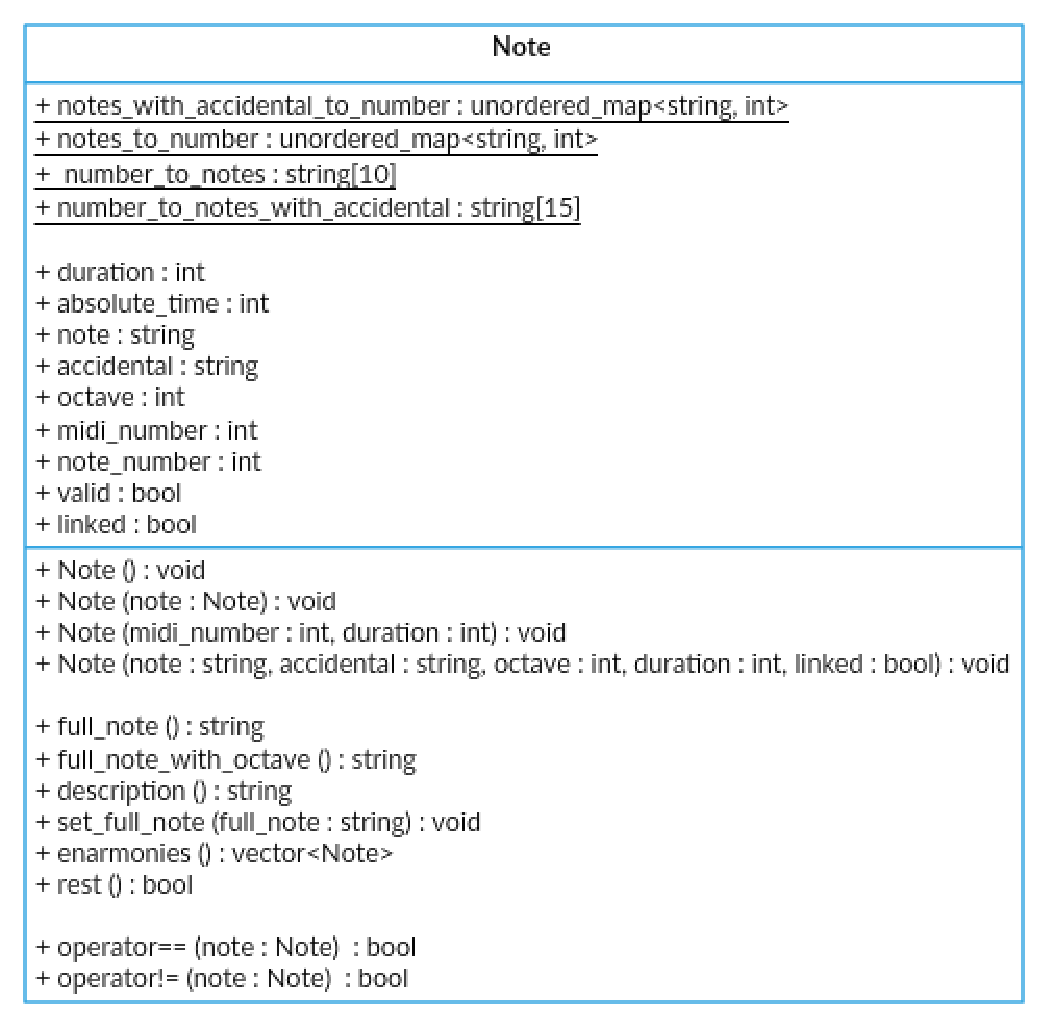
\includegraphics[scale=0.7]{figuras/noteclass.eps}
        \caption{Diagrama da Classe \texttt{Note}}
        \label{noteclass}
      \end{figure}

    \subsection[Classe \texttt{Compass Time}]{Classe \texttt{Compass Time}}

      A classe \texttt{Compass Time} armazena o tempo de compasso de uma música. Possui os seguintes atributos:

      \begin{enumerate}
        \item \texttt{times}: Número inteiro, armazena a quantidade de batidas que o compasso possui, por exemplo, em um compasso 3/4, ele armazena o valor 3.
        \item \texttt{base\_note}: Número inteiro, armazena qual é a figura musical base do compasso. Por exemplo, em um compasso 3/4, ele armazena o valor 4.
      \end{enumerate}

      Além dos atributos, essa classe possui dois métodos:

      \begin{enumerate}
        \item \texttt{base\_note\_duration()}: Retorna a duração da nota base.
        \item \texttt{compass\_duration()}: Retorna a duração total do compasso, multiplicando a duração da nota base pela quantidade de batidas.
      \end{enumerate}


      A Figura \ref{compasstimeclass} representa os atributos e métodos da classe.

      \begin{figure}[htb]
        \centering
        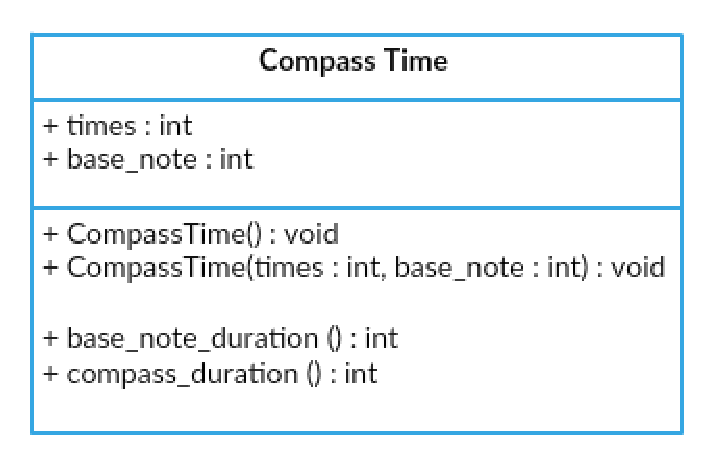
\includegraphics[scale=0.7]{figuras/compasstimeclass.eps}
        \caption{Diagrama da Classe \texttt{Compass Time}}
        \label{compasstimeclass}
      \end{figure}

    \subsection[Classe \texttt{Song}]{Classe \texttt{Song}}

      A classe \texttt{Song} armazena as informações básicas de uma música. Possui os seguintes atributos:

      \begin{enumerate}
        \item \texttt{notes}: Vetor que armazena as notas de uma música em ordem de execução.
        \item \texttt{scale}: Armazena a escala de uma música.
        \item \texttt{compass\_time}: Armazena o tempo de compasso de uma música, assumindo que não há troca de tempo no meio da canção.
      \end{enumerate}

      Em relação aos métodos, essa classe possui os seguintes:

      \begin{enumerate}
        \item \texttt{size()}: Retorna o número de notas da melodia.
        \item \texttt{back()}: Retorna a última nota da melodia ou uma nota inválida se a melodia não tiver nenhuma nota no estado atual.
        \item \texttt{size\_without\_rest()}: Retorna o número de notas da melodia sem notas de descanso que possam haver ao final desta.
        \item \texttt{trailing\_rests()}: Retorna o número de descansos ao final da melodia.

      \end{enumerate}

      A Figura \ref{songclass} representa os atributos e métodos da classe.

      \begin{figure}[htb]
        \centering
        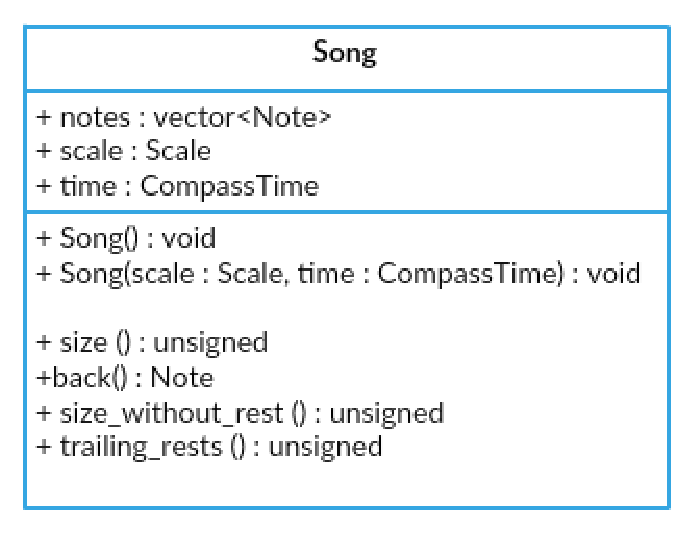
\includegraphics[scale=0.7]{figuras/songclass.eps}
        \caption{Diagrama da Classe \texttt{Song}}
        \label{songclass}
      \end{figure}

  \section[Módulo de Intervalos]{Módulo de Intervalos}

    Responsável pela geração e armazenamento de intervalos, este módulo possui a classe \texttt{Interval}.


    \subsection[Classe \texttt{Interval}]{Classe \texttt{Interval}}

      A classe \texttt{Interval} armazena intervalos e possui método para gerar uma nota a partir de outra e um intervalos. Ela possui os seguintes atributos:

      \begin{enumerate}
        \item \texttt{quantitative}: número inteiro, representa a classificação quantitativa do intervalo.
        \item \texttt{qualitative}: \texttt{string} que representa a classificação qualitativa do intervalo.
        \item \texttt{half\_tones}: número inteiro, representa a quantidade de semitons característica do intervalo.
        \item \texttt{direction}: Inteiro que indica se o intervalo é ascendente, descendente ou uníssono, no caso de intervalos melódicos.
      \end{enumerate}

      Excetuando-se métodos de impressão de atributos, a classe possui os seguintes métodos:

      \begin{enumerate}
        \item \texttt{is\_dissonant()}: retorna um booleano definindo se o intervalo é ou não dissonante, baseado nas regras do Contraponto Palestriniano.
        \item \texttt{is\_consonant()}: retorna um booleano definindo se o intervalo é ou não consonante.
        \item \texttt{ascendant()}: retorna um booleano definindo se o intervalo é ou não ascendente, definido a partir da primeira nota em relação à segunda.
        \item \texttt{descendant()}: retorna um booleano definindo se o intervalo é ou não ascendente.
        \item \texttt{ascendant\_or\_unison()}: retorna um booleano definindo se o intervalo é ou não ascendente ou uníssono.
        \item \texttt{descendant\_or\_unison()}: retorna um booleano definindo se o intervalo é ou não descendente ou uníssono.
        \item \texttt{interval\_to\_note()}: método de classe que retorna uma nota ao receber uma nota e um intervalo. A nota recebida é considerada a primeira ao utilizar a propriedade do intervalo ser ascendente ou descendente, pois uma nota e um intervalo sem atributo de ascendência pode gerar até duas notas, uma acima e outra abaixo da nota original.
      \end{enumerate}

      A Figura \ref{intervalclass} representa os atributos e métodos da classe.

      \begin{figure}[htb]
        \centering
        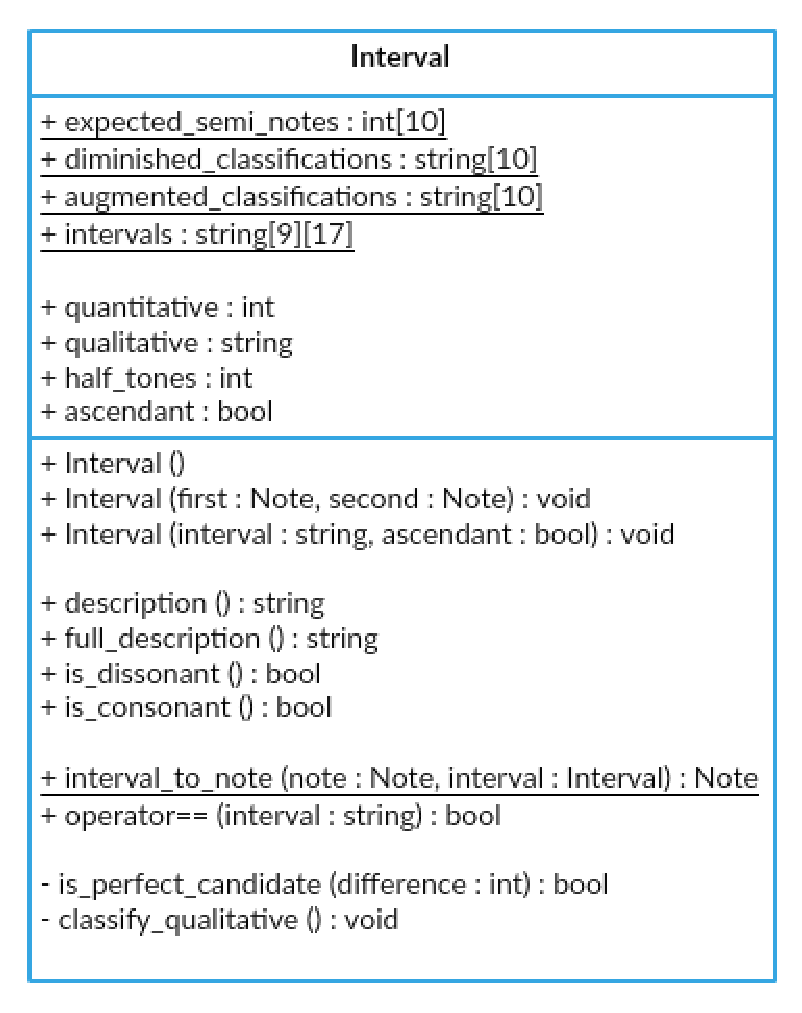
\includegraphics[scale=0.7]{figuras/intervalclass.eps}
        \caption{Diagrama da Classe \texttt{Interval}}
        \label{intervalclass}
      \end{figure}

  \section[Módulo de Escalas]{Módulo de Escalas}

    O módulo de escalas é responsável pela geração e armazenamento de escalas musicais. Ele possui uma classe, a \texttt{Scale}.

    \subsection[Classe \texttt{Scale}]{Classe \texttt{Scale}}

    A classe \texttt{Scale} armazena as notas de uma escala, possuindo apenas um atributo, um \texttt{set} de \texttt{strings} chamado \texttt{permitted\_notes} que define as notas permitidas para aquela escala. Além disso, ela possui os seguintes métodos:

    \begin{enumerate}
      \item \texttt{is\_valid\_note()}: recebe uma nota e diz se ela está ou não presente na escala.
      \item \texttt{interval\_to\_note\_on\_scale()}: método de classe que retorna uma nota, dado uma nota, um intervalo e uma escala. Retorna inválido se a nota não estiver presente na escala.
    \end{enumerate}


    A Figura \ref{scaleclass} representa os atributos e métodos da classe.

    \begin{figure}[htb]
      \centering
      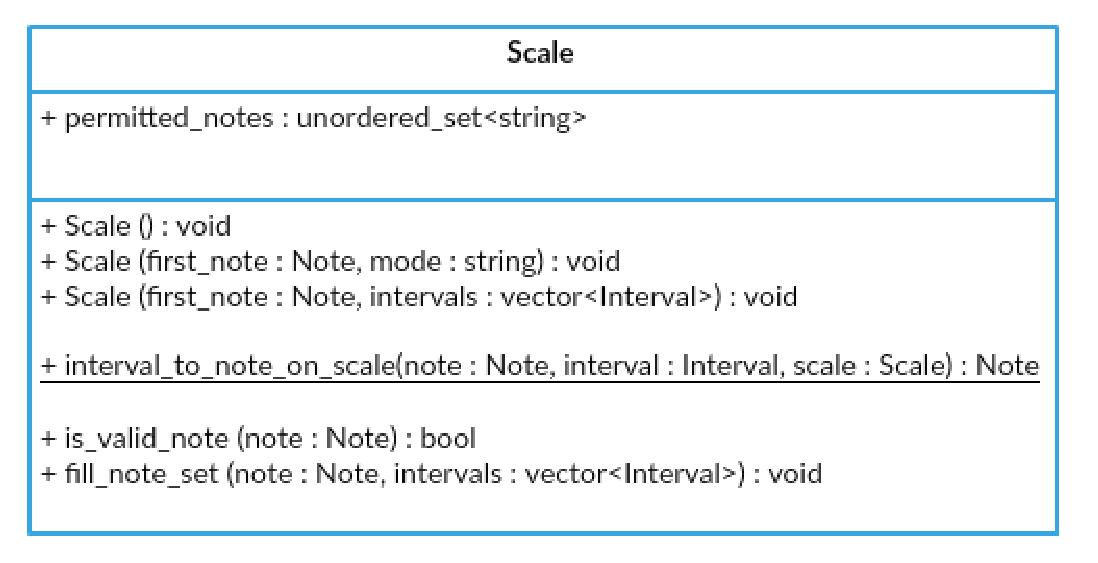
\includegraphics[scale=0.7]{figuras/scaleclass.eps}
      \caption{Diagrama da Classe \texttt{Scale}}
      \label{scaleclass}
    \end{figure}

  \section[Módulo de Contraponto]{Módulo de Contraponto}

    O módulo de contraponto é responsável pela geração de contrapontos. Utilizando todas as classes anteriormente citadas, possui cinco classes: \texttt{Counterpoint}, \texttt{First Species Counterpoint}, \texttt{Second Species Counterpoint}, \texttt{Third Species Counterpoint} e \texttt{Fourth Species Counterpoint}.

    \subsection[Classe \texttt{Counterpoint}]{Classe \texttt{Counterpoint}}

    A classe \texttt{Counterpoint} funciona como uma biblioteca e não possui atributos de instância. Inicialmente utilizada para a implementação do contraponto de primeira espécie, atualmente possui atributos estáticos como a matriz \textit{DP} utilizada para armazenar estados da solução e um ponteiro para \texttt{Song} utilizado para guardar referência para o \textit{cantus firmus} durante toda a solução, possui ainda o método ad-hoc de geração de contrapontos e o método \texttt{analyse\_and\_add\_interval()}.

    Além disso, possui o método \texttt{add\_trailing\_rests()} que adiciona descanso ao final do contraponto que não foram utilizados ao gerar a solução final. Esse método é importante para os algoritmos de segunda e terceira espécie, em que a última nota que não é descanso possui apenas uma nota no mesmo tempo no contraponto. O método \texttt{is\_thesis()} diz se uma nota está ou não no tempo forte do compasso dada sua posição, utilizado para utilizar ou não dissonâncias em dados momentos da solução nos algoritmos de segunda a quarta espécie.

    A solução inicialmente concebida utiliza um algoritmo de seleção aleatório. Iniciando na primeira nota do \textit{cantus firmus}, monta-se um vetor de notas possíveis para o contraponto em seu estado atual, escolhe-se aleatoriamente uma das notas do vetor e a insere no vetor do contraponto, seguindo para a próxima nota. O vetor de notas possíveis era montado de acordo com as regras do contraponto de primeira espécie anteriormente citadas.

    O problema dessa solução era o fato de escolher randomicamente um caminho e não explorar os outros, o que podia levar a um caminho que não levava a uma solução. Para contornar isso, o algoritmo era rodado diversas vezes até se encontrar uma solução. Contudo, em músicas maiores, o tempo de execução chegava a dois minutos ou mais, e em músicas impossíveis de se gerar contraponto, o algoritmo entrava em \textit{loop} infinito.

    Essa classe é utilizada como classe pai das classes dos contrapontos de primeira a quarta espécie. A Figura \ref{counterpointclass} apresenta os atributos e métodos da classe.

    \begin{figure}[htb]
      \centering
      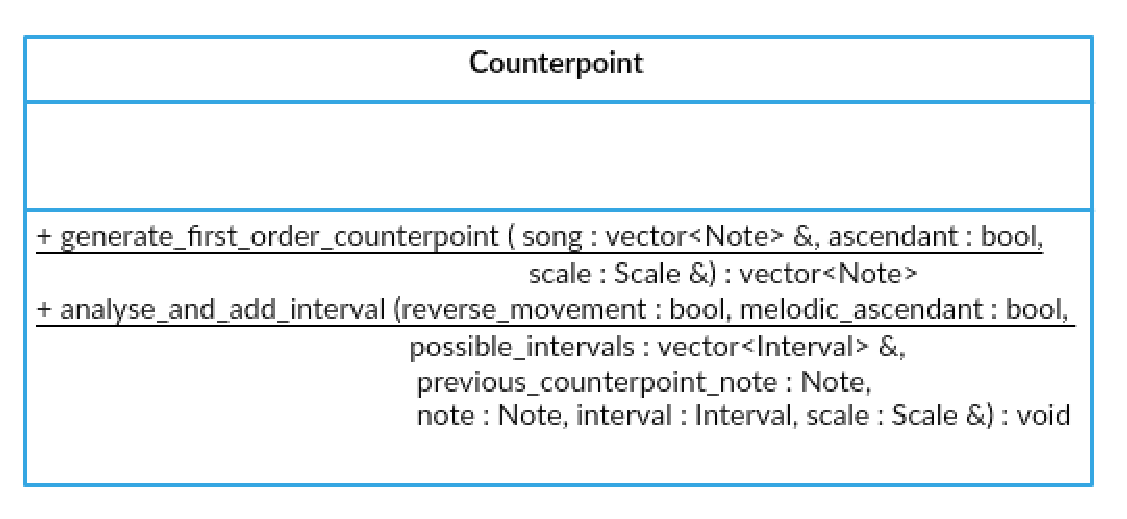
\includegraphics[scale=0.7]{figuras/counterpointclass.eps}
      \caption{Diagrama da Classe \texttt{Counterpoint}}
      \label{counterpointclass}
    \end{figure}

    \subsection[Classe \texttt{First Species Counterpoint}]{Classe \texttt{First Species Counterpoint}} \label{ssec:fec}

      A classe \texttt{First Species Counterpoint} herda da classe \texttt{Counterpoint} e é uma biblioteca, possuindo métodos de classe. Ela possui os seguintes métodos:

      \begin{enumerate}
        \item \texttt{dfs\_generate\_counterpoint()}: recebe uma instância de \texttt{Song}, um booleano que define se o contraponto será superior ou inferior e os números de terças e sextas paralelas e movimentos paralelos permitidos. Retorna um vetor de notas correspondente ao contraponto gerado.
        \item \texttt{solve()}: Método recursivo que executa a busca completa para gerar contrapontos. Tem como parâmetros a posição atual no \textit{cantus firmus}, o número atual de terças ou sextas paralelas, o número de movimentos paralelos já ocorridos, a instância do \textit{cantus firmus} e da proposta de contraponto atual passadas por referência e um booleano indicando se o contraponto é inferior ou superior.
        \item \texttt{analyse\_and\_add\_interval()}: método de análise de notas para inserção no contraponto, avalia regras como tamanho do salto e natureza do movimento (reverso ou não) e adiciona o intervalo sugerido na lista de possíveis intervalos caso ele atenda às regras estabelecidas.
      \end{enumerate}

      A Figura \ref{firstspeciescounterpointclass} apresenta os métodos e atributos da classe.

      \begin{figure}[htb]
        \centering
        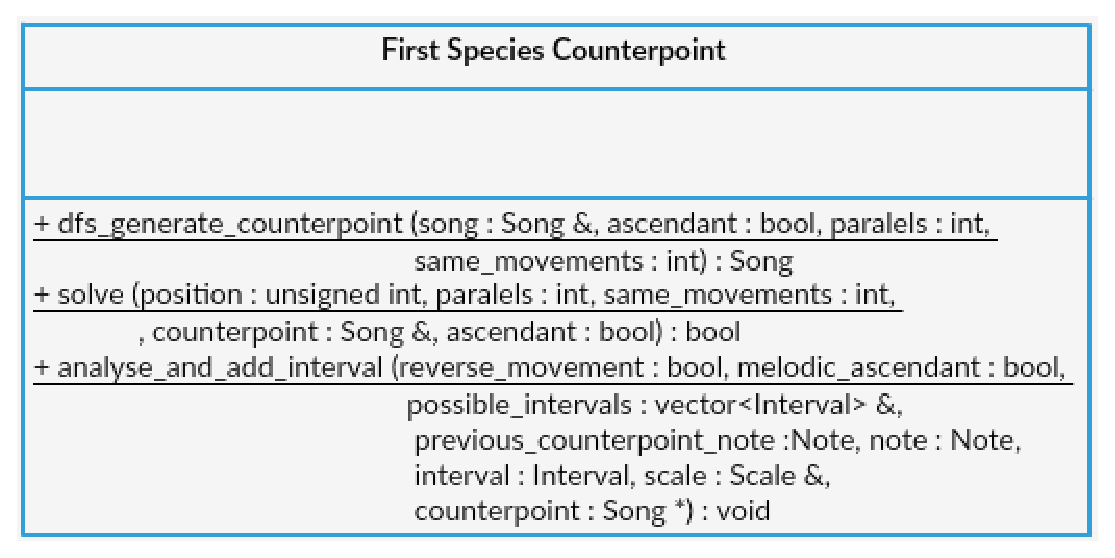
\includegraphics[scale=0.7]{figuras/firstspeciescounterpointclass.eps}
        \caption{Diagrama da Classe \texttt{First Species Counterpoint}}
        \label{firstspeciescounterpointclass}
      \end{figure}

    \subsection[Classes \texttt{Second Species Counterpoint} a \texttt{Fourth Species Counterpoint}]{Classes \texttt{Second Species Counterpoint} a \texttt{Fourth Species Counterpoint}}

      A classes de \texttt{Second Species Counterpoint}, \texttt{Third Species Counterpoint} e \texttt{Fourth Species Counterpoint} herdam da classe \texttt{Counterpoint} e possuem os mesmos métodos apresentados em \ref{ssec:fec}. A Figuras \ref{secondspeciescounterpointclass}, \ref{thirdspeciescounterpointclass} e \ref{thirdspeciescounterpointclass} apresentam os métodos e atributos das classes.

      \begin{figure}[htb]
        \centering
        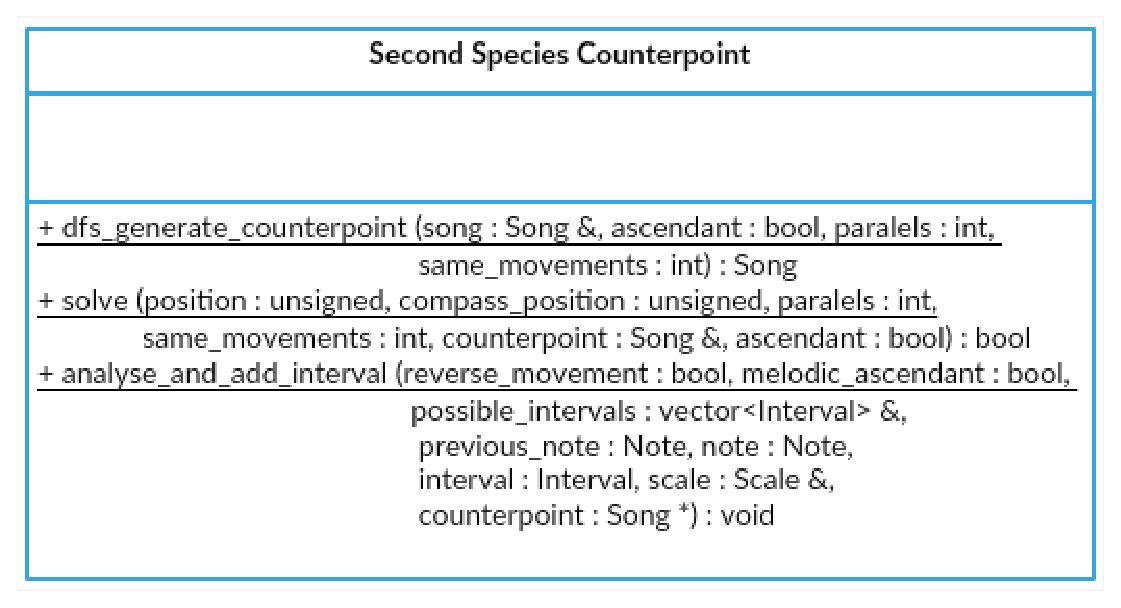
\includegraphics[scale=0.7]{figuras/secondspeciescounterpointclass.eps}
        \caption{Diagrama da Classe \texttt{Second Species Counterpoint}}
        \label{secondspeciescounterpointclass}
      \end{figure}

    \begin{figure}[htb]
      \centering
      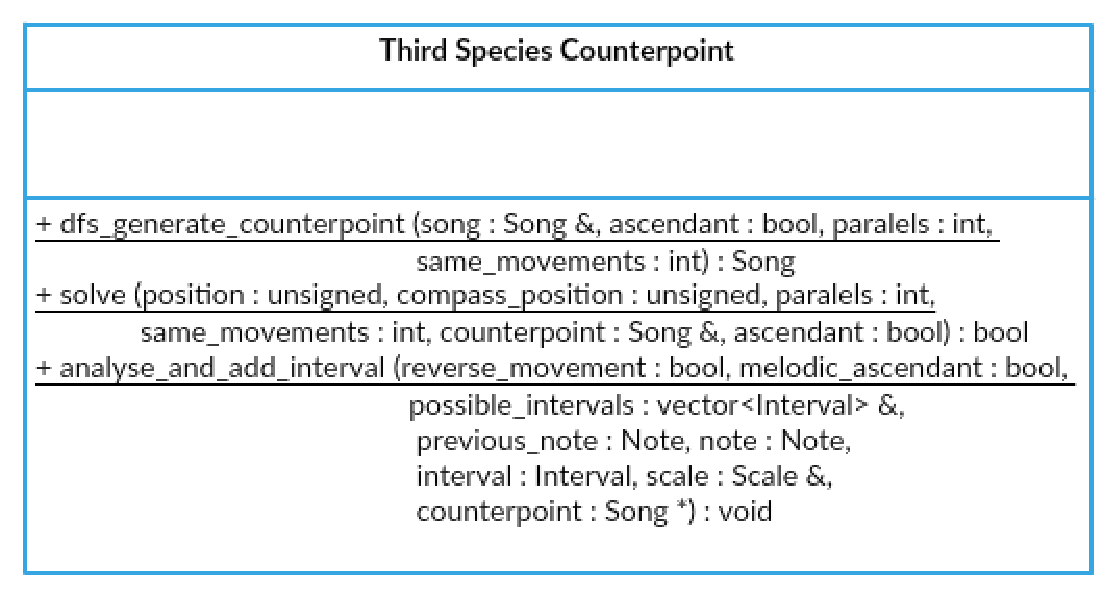
\includegraphics[scale=0.7]{figuras/thirdspeciescounterpointclass.eps}
      \caption{Diagrama da Classe \texttt{Third Species Counterpoint}}
      \label{thirdspeciescounterpointclass}
    \end{figure}

    \begin{figure}[htb]
      \centering
      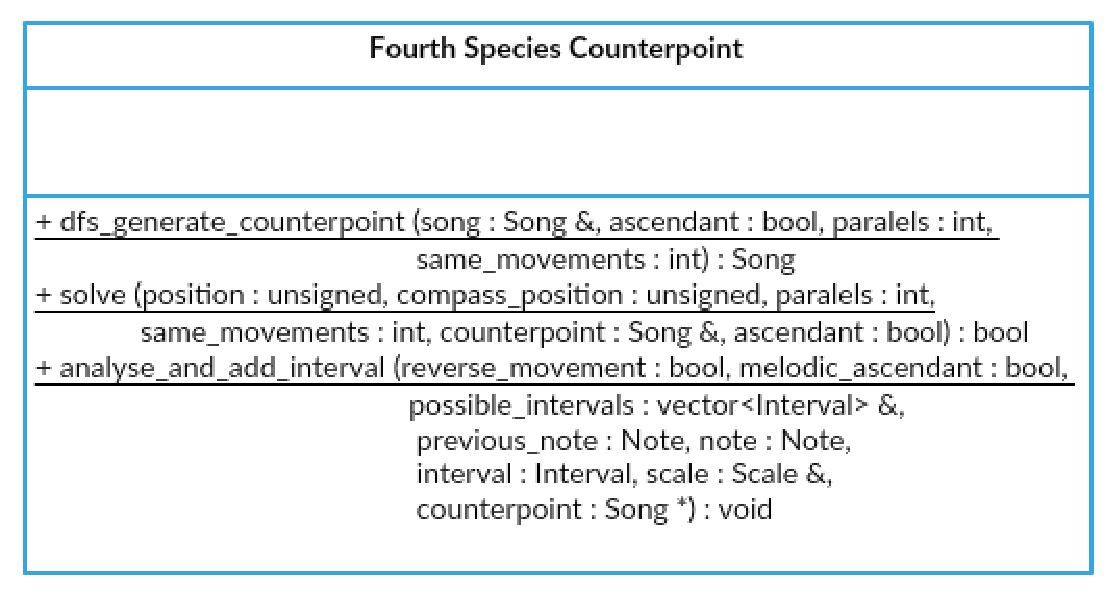
\includegraphics[scale=0.7]{figuras/fourthspeciescounterpointclass.eps}
      \caption{Diagrama da Classe \texttt{Fourth Species Counterpoint}}
      \label{fourthspeciescounterpointclass}
    \end{figure}

    O método que retorna o vetor de contrapontos encapsula a solução e chama o método recursivo. O algoritmo possui o seguinte funcionamento: iniciando na primeira posição do \textit{cantus firmus}, o estado da DP é definido por cinco parâmetros: posição, posição no compasso, número MIDI da nota atual, número de terças ou sextas paralelas anteriormente executadas e número de movimentos paralelos.

    A transição ocorre após a geração do vetor de notas possíveis, de acordo com as regras do contraponto. Para cada nota do vetor de intervalos, adiciona-se a nota ao final do vetor de contrapontos se a inserção dela não fizer ultrapassar o número de terças, sextas e movimentos paralelos.

    Após a adição da nota, o método \texttt{solve()} é chamado para a posição mais um, com o número de terças, sextas e movimentos paralelos atualizados. O retorno do método \texttt{solve()} é um booleano que indica se há um contraponto válido ao explorar aquele caminho. Portanto, se o retorno for \texttt{false}, a nota adicionada no final do vetor de contrapontos é removida e a próxima nota do vetor de notas possíveis é testada. Contudo, se o retorno for \texttt{true}, ela também retorna \texttt{true} e não remove a nota atual, mantendo o vetor de contraponto gerado como solução. Se a análise das notas não adicionar nenhuma nota no vetor de notas possíveis, o método retorna também \texttt{false}.

    Vale ressaltar que o vetor de notas possíveis é embaralhado aleatoriamente para garantir uma solução diferente a cada execução do algoritmo. Além disso, primeiro adiciona-se as notas que geram movimento contrário, embaralha-se a primeira parte do vetor, em seguida, adiciona-se as notas que geram movimento paralelo e embaralha-se a segunda parte do vetor. Isso é feito para que a solução priorize o menor número de movimentos paralelos possível.

    O caso-base da DP é quando a posição é maior que o tamanho do \textit{cantus firmus}. Se o algoritmo chegar a essa posição, significa que a proposta de contraponto atual é um contraponto válido, portanto, retorna-se \texttt{true}.

    Para que o algoritmo funcione efetivamente como uma DP, é utilizado um vetor de memorização booleano de cinco dimensões, uma para cada estado. A primeira possui 151 espaços, permitindo que um contraponto seja gerado para um \textit{cantus firmus} com, no máximo, 151 notas. A segunda dimensão possui 4 espaços e indica a posição do contraponto em relação à nota atual, especialmente utilizado em contrapontos de segunda a quarta espécie, em que cada nota do \textit{cantus firmus} possui duas ou quatro notas no tempo equivalente no contraponto. Em contrapontos de primeira espécie, esse valor é sempre 0, em contrapontos de segunda e quarta espécie vai de 0 a 1 e em contrapontos de terceira espécie vai de 0 a 4. A terceira dimensão possui 90 espaços e representa o número MIDI da nota atual e cobre as 88 primeiras notas do piano. A quarta dimensão possui 5 espaços e cobre as 4 terças ou sextas paralelas seguidas permitidas pelo algoritmo. A quinta dimensão representa o número de movimentos paralelos que aconteceram durante o contraponto, possui 601 espaços pois o máximo de movimentos paralelos permitidos pelo algoritmo é a música completa multiplicada por 4, que é o máximo número de notas em um contraponto de terceira espécie.

    Utilizando o vetor de DP, ele inicia todas as posições com \texttt{true}. Quando o algoritmo encontra um estado que é não possui solução, memoriza como \texttt{false} na posição do vetor de DP que representa aquele e todas as posteriores consultas àquele estado retornam falso sem explorar esse candidato de solução novamente.

    Um exemplo é se o algoritmo definir que o estado atual -- na posição 10, na terceira nota do contraponto para aquela nota do \textit{cantus firmus}, na nota C4 (\texttt{midi\_number} 60), com 2 terças ou sextas paralelas e 13 movimentos paralelos -- não é uma solução, memoriza-se \texttt{false} em dp[10][2][60][2][13]. Na próxima consulta a esse estado, retorna falso imediatamente sem explorar. Memorizar estados que retornam \texttt{true} é irrelevante pois o primeiro estado completo que chega ao final retornando \texttt{true} é definido como a solução.

    A Figura \ref{algoritmo} apresenta o fluxograma do algoritmo.

    \begin{figure}[htb]
      \centering
      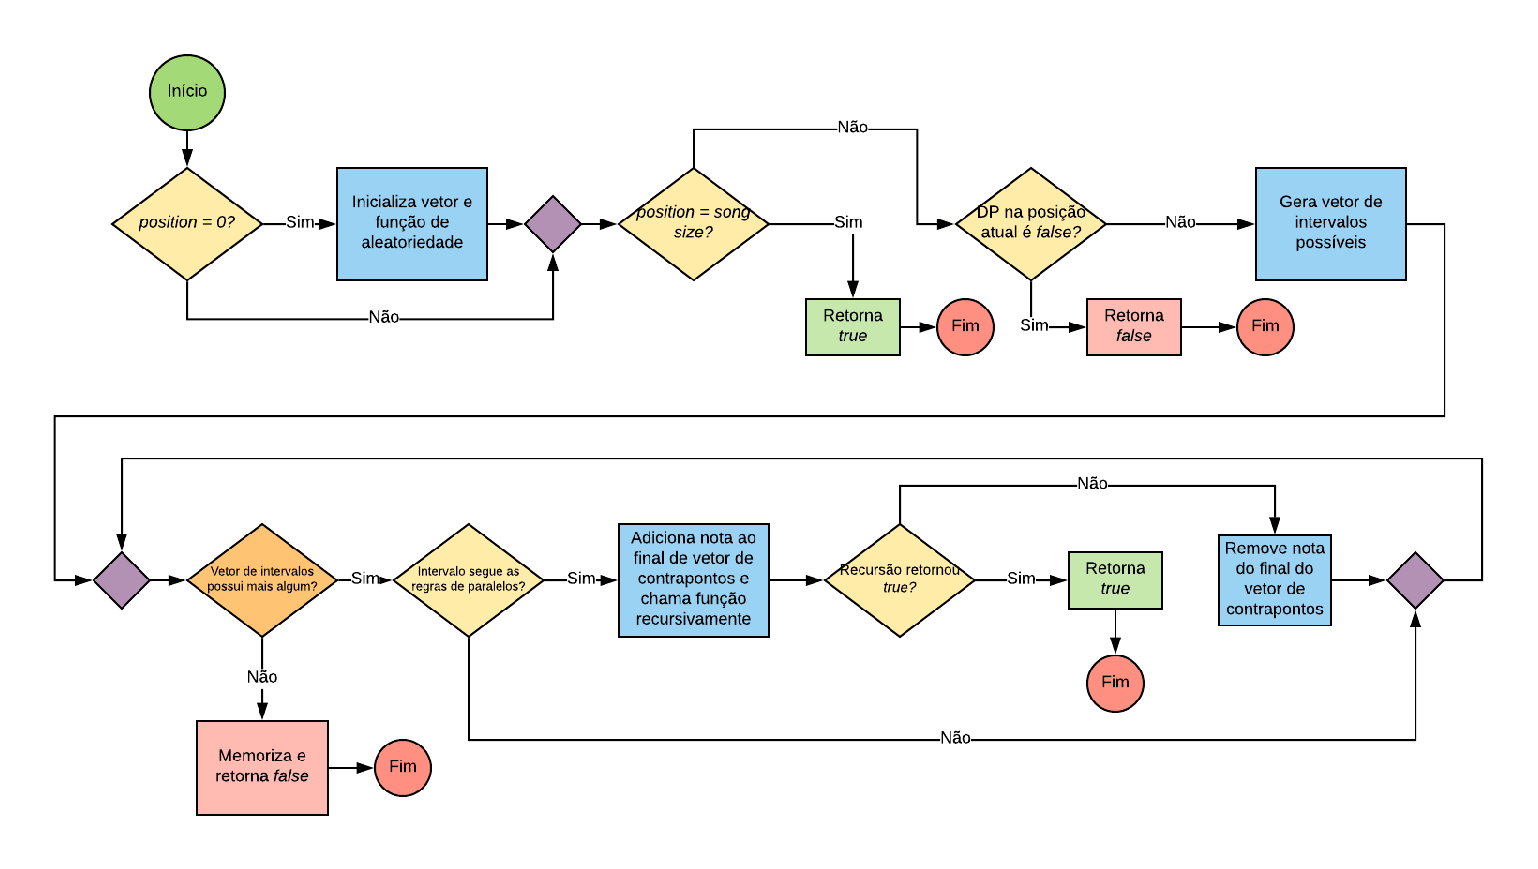
\includegraphics[scale=0.6]{figuras/algoritmo.eps}
      \caption{Algoritmo de Geração de Contrapontos}
      \label{algoritmo}
    \end{figure}


  \section[\texttt{Main}]{\texttt{Main}}

    A \texttt{main()} é a função principal que executa o programa. Nela o arquivo .ly é lido -- primeiramente lendo a tônica e o modo da escala, seguido pela leitura do ritmo. Após isso, cada nota é lida e convertida para uma instância de \texttt{Note} por meio da \texttt{Song Reader}. Para efeitos de teste, atualmente, os intervalos melódicos são calculados e impressos no terminal, bem como a transformação de \texttt{Note} para \texttt{string} novamente.

    Após a leitura, o algoritmo de contraponto é executado. É gerado um vetor de notas com o contraponto de primeira espécie. Esse vetor é impresso no terminal em notação musical padrão e em notação específica do Lilypond para fácil transferência do contraponto para o arquivo original.

  \section[Módulo de Construção do MIDI]{Módulo de Construção do MIDI}

    O módulo de construção do MIDI é responsável por encapsular a solução de leitura de arquivos Lilypond e geração de um arquivo Lilypond com o contraponto gerado adicionado a ele. Além disso, ele utiliza as bibliotecas do Lilypond para gerar a partitura e o arquivo .mid a partir do arquivo gerado. Esse módulo é constituído pelas classes \texttt{Song Reader} e \texttt{Ly Parser} e pela aplicação \texttt{Counterpoint Generator} desenvolvida em \textit{Ruby On Rails}.

    \subsection[Classe \texttt{Song Reader}]{Classe \texttt{Song Reader}}

      A classe \texttt{Song Reader} é responsável pelo \textit{parser} de \texttt{string} representando notas em formato Lilypond para instâncias da classe \texttt{Note} e vice-versa. Sem a necessidade de atributos e com apenas métodos de classe, a classe age como uma biblioteca, sendo utilizada sem instanciação. Ela possui os seguintes métodos:


      \begin{enumerate}
        \item \texttt{string\_to\_note()}: retorna uma instância de \textit{Note} ao receber uma \texttt{string} e uma nota. A nota recebida como parâmetro é a nota anterior, pois o formato Lilypond omite a duração da nota se for a mesma da anterior.
        \item \texttt{note\_to\_string()}: retorna uma \texttt{string} que representa uma nota em formato Lilypond ao receber um objeto \texttt{Note}.
        \item \texttt{scale\_to\_string()}: retorna uma instância da \texttt{Scale} ao receber uma \texttt{string}.
        \item \texttt{string\_to\_scale()}: retorna uma \texttt{string} que representa escalas no formato Lilypond ao receber um objeto da classe \texttt{Scale}.
        \item \texttt{compass\_time\_to\_string()}: retorna uma instância da \texttt{CompassTime} ao receber uma \texttt{string}.
        \item \texttt{string\_to\_compass\_time()}: retorna uma \texttt{string} que representa ritmo no formato Lilypond ao receber um objeto da classe \texttt{CompassTime}.
        \item \texttt{song\_clef\_to\_string()}: retorna uma \texttt{string} que define em qual clave a melodia deve ser impressa baseada no valor médio da nota -- uma melodia com notas mais agudas é impressa na clave de sol e uma melodia com notas mais baixas é impressa na classe de fá.
        \item \texttt{song\_to\_voice\_string()}: retorna uma \texttt{string} que representa a voz do contraponto no Lilypond, a voz é impressa com clave, escala e ritmo seguidos das notas musicais.
        \item \texttt{new\_staff\_string()}: retorna uma \texttt{string} que define uma nova voz no arquivo Lilypond, sendo essa voz nomeada de \texttt{CounterpointVoice}.
        \item \texttt{midi\_indicator()}: retorna uma \texttt{string} que indica que o lilypond em que ela for adicionada deve gerar um arquivo MIDI além do PDF da partitura.
        \item \texttt{msb()}: retorna o bit mais significativo, utilizado no cálculo da figura musical baseado na duração da nota. Quanto maior for o valor da figura musical, menor a duração, mas pontos de aumento podem modificar a duração da nota e o bit mais significativo é usado para inferir o valor da figura musical, pois as figuras sem pontos de aumento sempre geram durações representadas por potências de 2.
        \item \texttt{number\_of\_on\_bits()}: retorna o número de bits ligados de um inteiro, útil pois deriva o número de pontos de aumento de uma nota (para gerar a \texttt{string}) a partir da representação binária da duração.
      \end{enumerate}

      A Figura \ref{songreaderclass} representa os métodos da classe.

      \begin{figure}[htb]
        \centering
        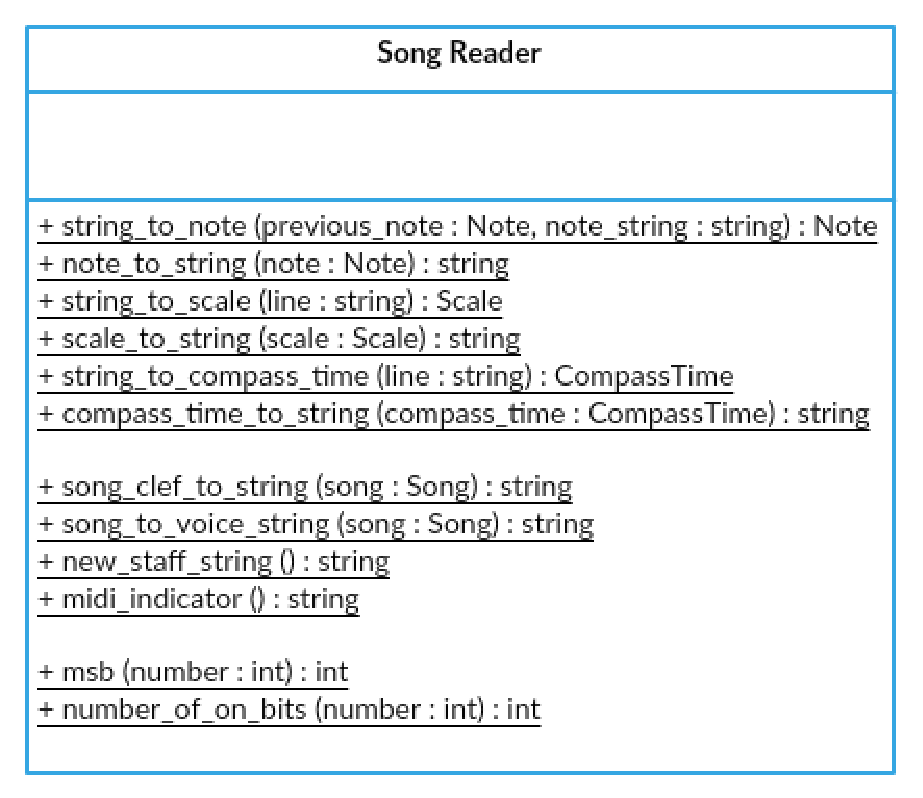
\includegraphics[scale=0.8]{figuras/songreaderclass.eps}
        \caption{Diagrama da Classe \texttt{Song Reader}}
        \label{songreaderclass}
      \end{figure}

    \subsection[Classe \texttt{Ly Parser}]{Classe \texttt{Ly Parser}}


      A classe \texttt{Ly Parser} é responsável pela leitura de um arquivo Lilypond completo e a geração de um novo arquivo Lilypond completo com o contraponto inserido. Para isso, ela primeiramente lê o arquivo original e gera um arquivo simplificado a partir dele. Após isso, ela lê os dados do arquivo simplificado utilizando a classe \texttt{Song Reader}. Após a geração do contraponto, ela adiciona o contraponto ao arquivo original, gerando um novo arquivo Lilypond. Ela possui os seguintes métodos:

      \begin{enumerate}
        \item \texttt{read\_file()}: lê um arquivo Lilypond simplificado em formato pré-estabelecido e retorna uma instância da classe \texttt{Song} com escala, ritmo e notas lidas.
        \item \texttt{convert\_file\_to\_simple\_format()}: Recebe o caminho de um arquivo Lilypond completo e gera um arquivo Lilypond simplificado em outro caminho especificado.
        \item \texttt{add\_counterpoint\_to\_lilypond()}: Recebe um contraponto gerado, o caminho do arquivo original e gera um novo arquivo Lilypond com a voz do contraponto gerado adicionada.
      \end{enumerate}

      A Figura \ref{lyparserclass} apresenta os métodos e atributos da classe.

      \begin{figure}[htb]
        \centering
        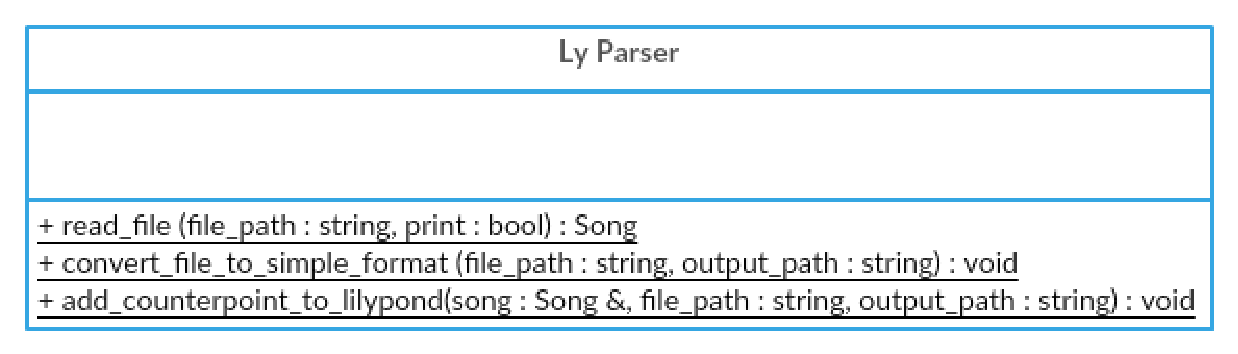
\includegraphics[scale=0.7]{figuras/lyparserclass.eps}
        \caption{Diagrama da Classe \texttt{Ly Parser}}
        \label{lyparserclass}
      \end{figure}

    \subsection[\texttt{Counterpoint Generator}]{\texttt{Counterpoint Generator}}

      O \texttt{Counterpoint Generator} é uma aplicação \textit{web} desenvolvida em \textit{Ruby On Rails}. Nela, seleciona-se o arquivo Lilypond escolhido para se gerar um contraponto, a espécie de contraponto e se ele será inferior ou superior. Utilizando o executável do algoritmo em C++, o contraponto é gerado e o novo arquivo Lilypond é utilizado para gerar a partitura em PDF e o arquivo .mid. A aplicação compacta o arquivo Lilypond, o PDF e o MIDI e os envia para o usuário.


            A Figura \ref{counterpointgenerator} apresenta o acesso ao \textit{front-end} da aplicação.

            \begin{figure}[htb]
              \centering
              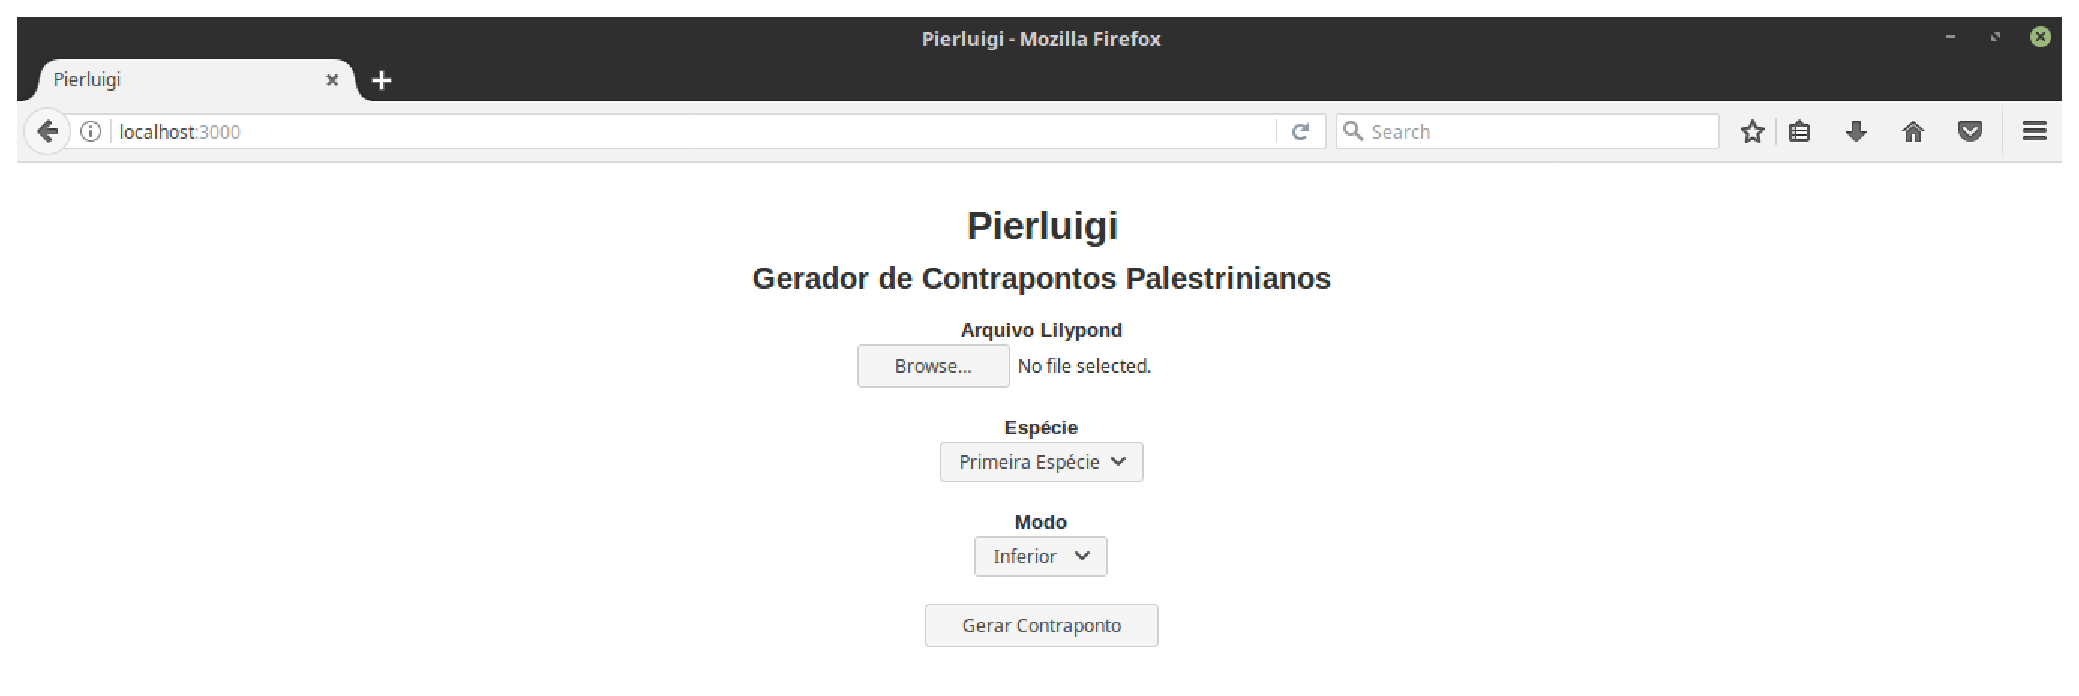
\includegraphics[scale=0.45]{figuras/counterpointgenerator.eps}
              \caption{Página \textit{web} do \textit{Pierluigi}}
              \label{counterpointgenerator}
            \end{figure}

  \section[Experimentos]{Experimentos}

    Para validar o algoritmo construído, foram feitos experimentos em músicas pequenas para melhor análise do resultado. O teste da execução do algoritmo foi feito utilizando várias músicas. Serão apresentados os testes feitos com a música infantil \textit{Twinkle Twinkle Little Star}. O código-fonte da solução está disponível em \textit{\url{https://github.com/joao18araujo/pierluigi}}, o código-fonte do \textit{front-end} da aplicação está disponível em \textit{\url{https://github.com/joao18araujo/pierluigi_frontend}}.

    Todos os módulos implementados possuem testes automatizados. Para isso, utilizou-se a biblioteca Catch2. Para garantir a corretude dos testes durante o desenvolvimento, foi utilizada uma ferramenta de integração contínua no repositório. O resultado dos testes pode ser observado em \textit{\url{https://travis-ci.org/joao18araujo/pierluigi}}.

    A música original pode ser observada em formato Lilypond e em partitura no Código \ref{twinklecode} e na Figura \ref{twinkleoriginal}, respectivamente.

    \begin{lstlisting}[language={C++}, caption={\textit{Twinkle Twinkle Little Star}}, label={twinklecode}]
    \key c \major
    \time 4/4
    c''4 c'' g'' g''
    a'' a'' g''2
    f''4 f'' e'' e''
    d'' d'' c''2
    g''4 g'' f'' f''
    e'' e'' d''2
    g''4 g'' f'' f''
    e'' e'' d''2
    c''4 c'' g'' g''
    a'' a'' g''2
    f''4 f'' e'' e''
    d'' d'' c''2
    \end{lstlisting}

    \begin{figure}[htb]
      \centering
      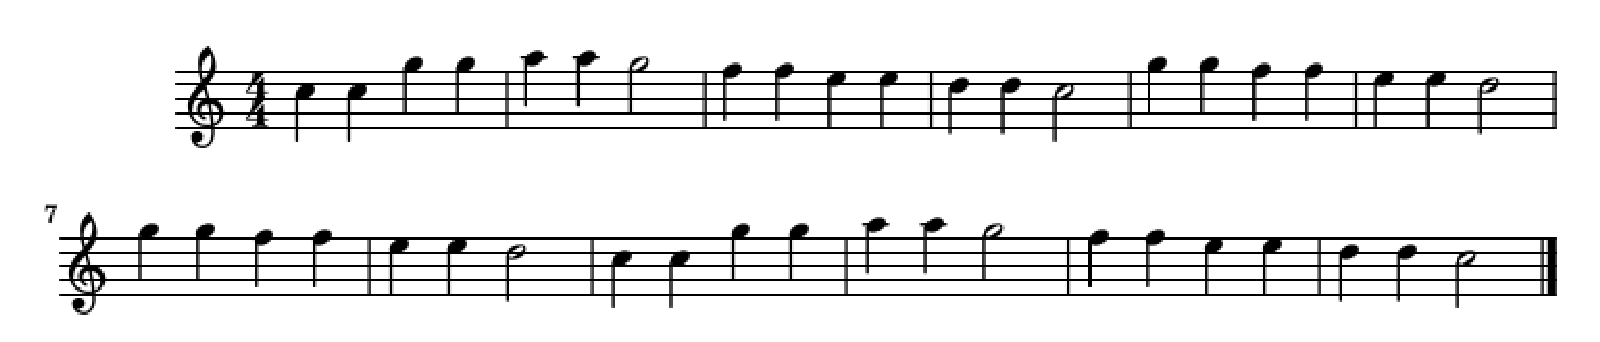
\includegraphics[scale=0.6]{figuras/twinkleoriginal.eps}
      \caption{Partitura de \textit{Twinkle Twinkle Little Star}}
      \label{twinkleoriginal}
    \end{figure}

    Após a execução do algoritmo para contraponto de primeira espécie, o contraponto gerado pode ser visto em partitura na Figura \ref{cont1.2}.

    \begin{figure}[htb]
      \centering
      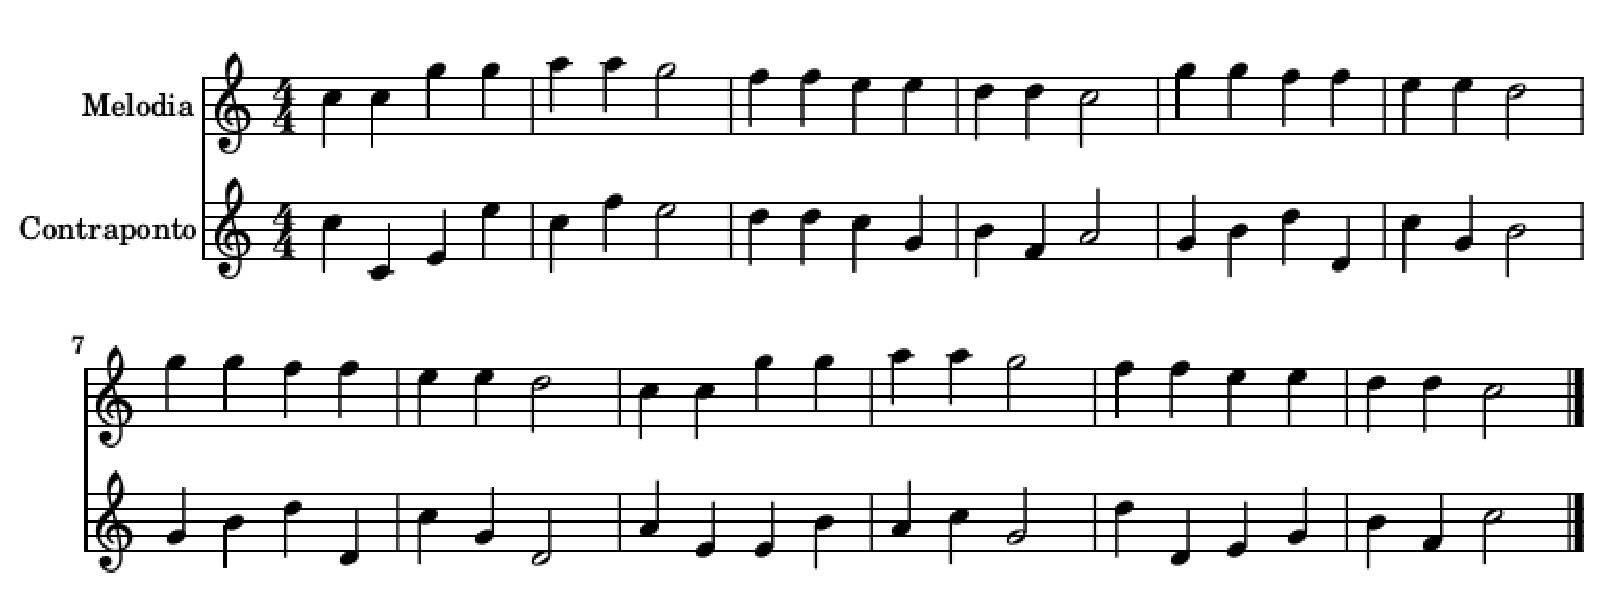
\includegraphics[scale=0.6]{figuras/cont1.2.eps}
      \caption{Partitura do contraponto de primeira espécie gerado}
      \label{cont1.2}
    \end{figure}

    Após a execução do algoritmo para contraponto de segunda espécie, o contraponto gerado pode ser visto em partitura na Figura \ref{cont2.2}.

        \begin{figure}[htb]
          \centering
          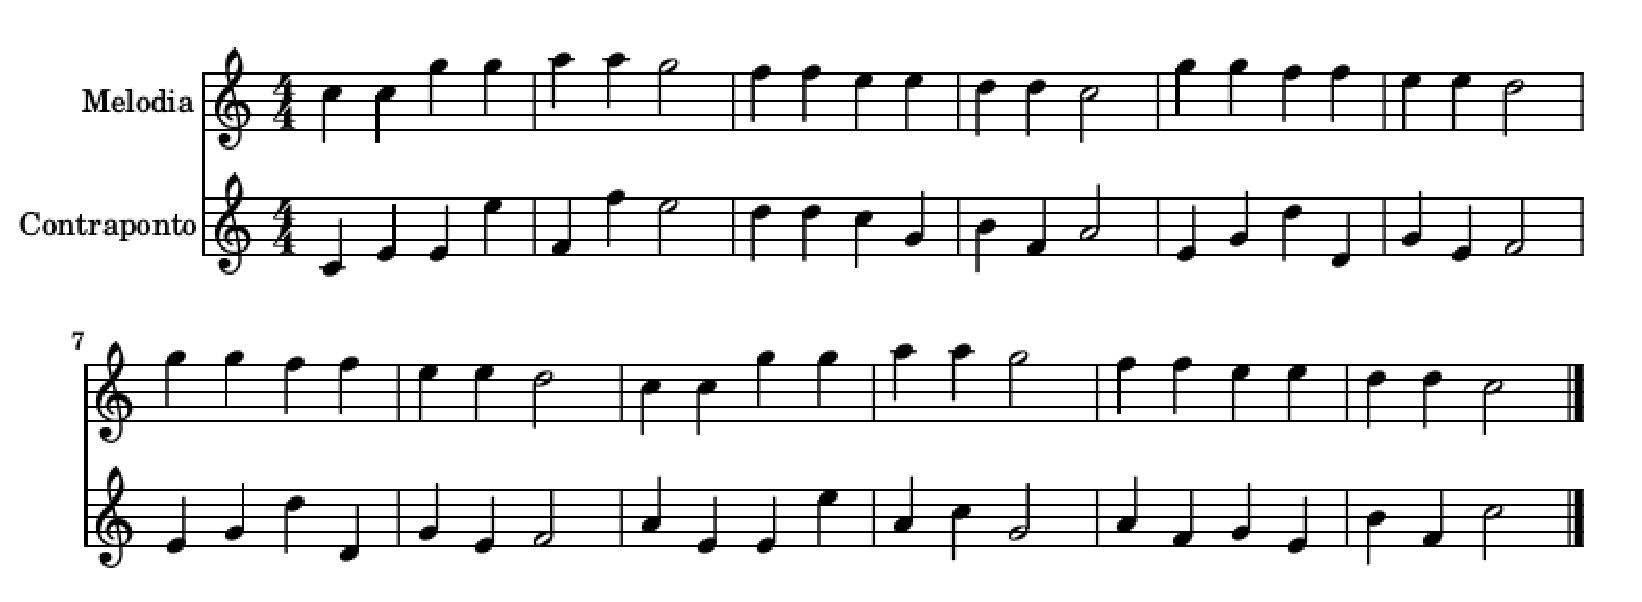
\includegraphics[scale=0.6]{figuras/cont2.2.eps}
          \caption{Partitura do contraponto de segunda espécie gerado}
          \label{cont2.2}
        \end{figure}

    Após a execução do algoritmo para contraponto de terceira espécie, o contraponto gerado pode ser visto em partitura na Figura \ref{cont3.2}.

    \begin{figure}[htb]
      \centering
      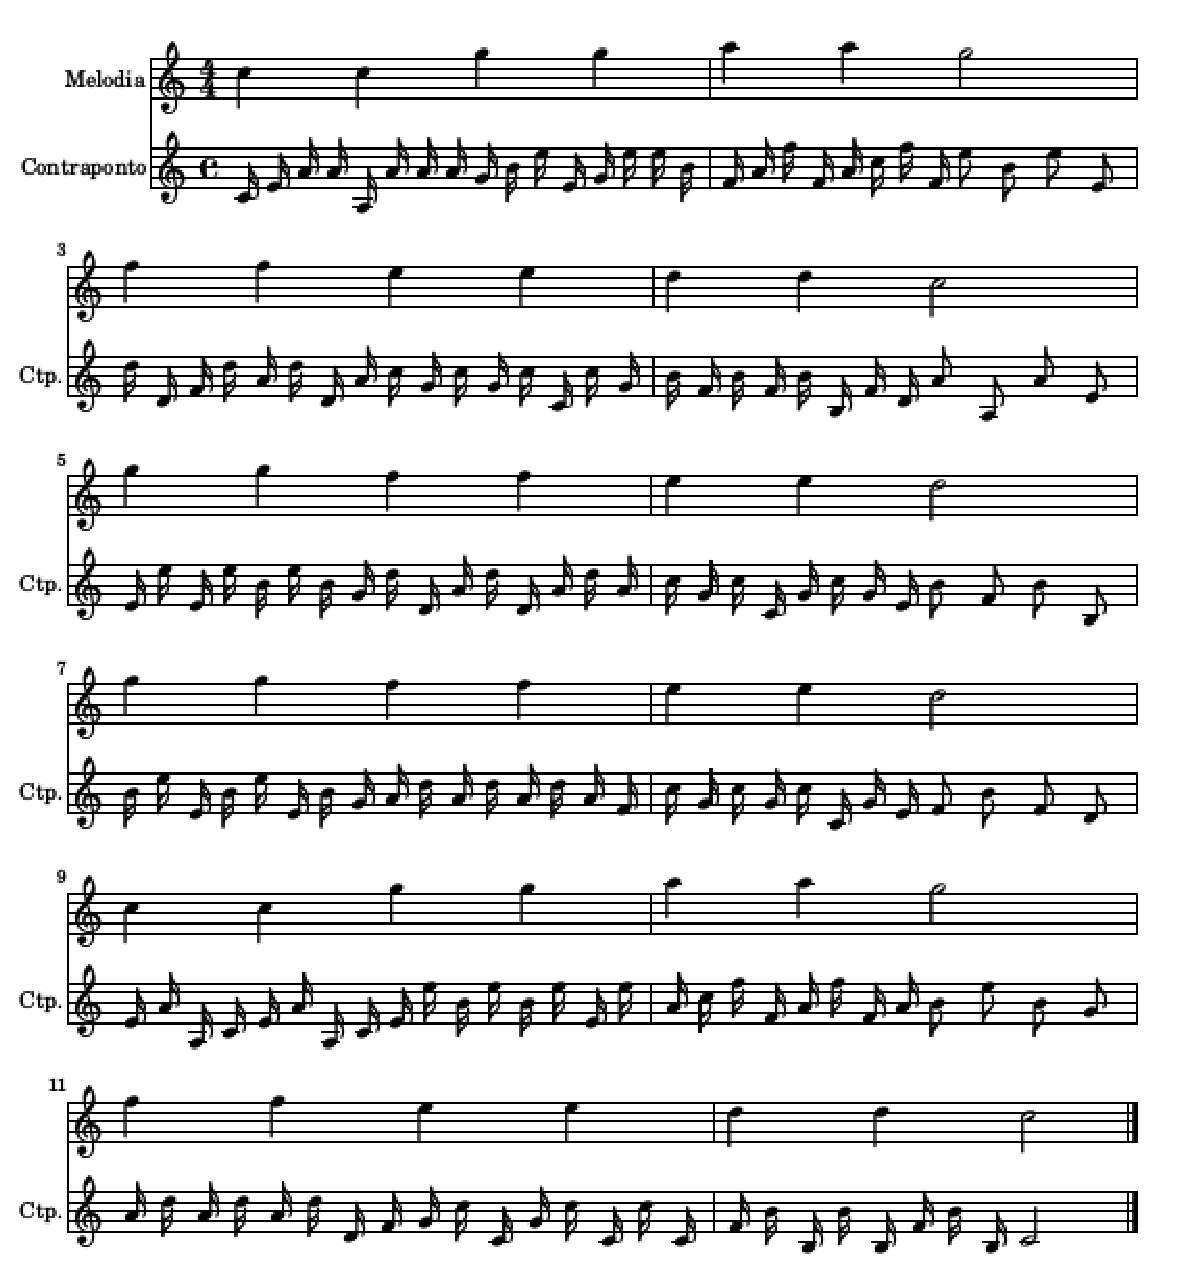
\includegraphics[scale=0.6]{figuras/cont3.2.eps}
      \caption{Partitura do contraponto de terceira espécie gerado}
      \label{cont3.2}
    \end{figure}

    Após a execução do algoritmo para contraponto de quarta espécie, o contraponto gerado pode ser visto em partitura na Figura \ref{cont4.2}.

    \begin{figure}[htb]
      \centering
      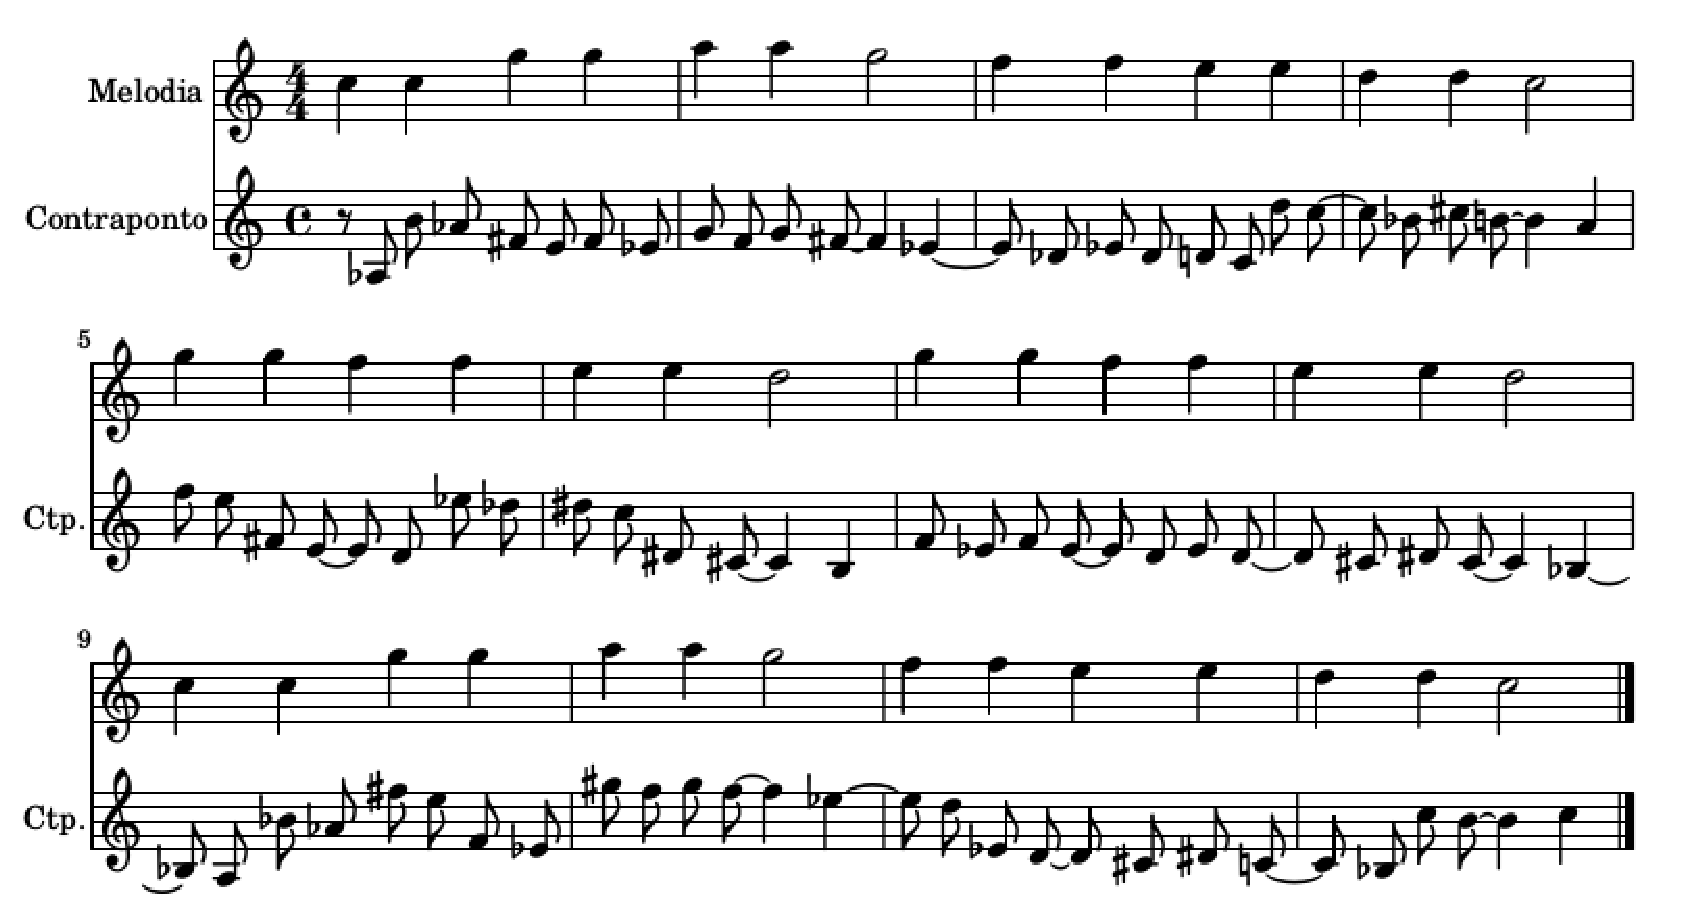
\includegraphics[scale=0.6]{figuras/cont4.2.eps}
      \caption{Partitura do contraponto de quarta espécie gerado}
      \label{cont4.2}
    \end{figure}
